\documentclass{standalone}
\usepackage{tikz}
\usetikzlibrary{positioning}

\begin{document}

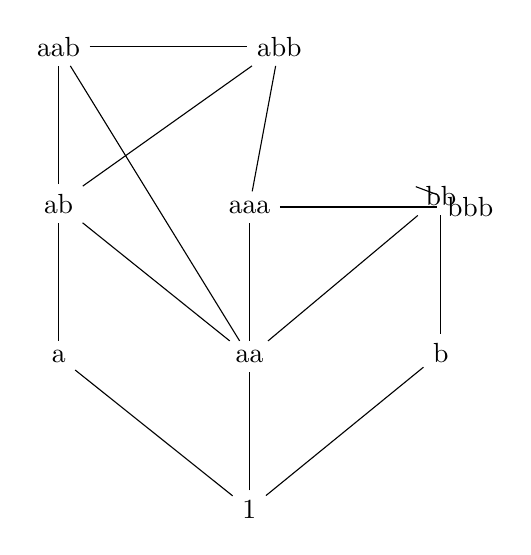
\begin{tikzpicture}[node distance=1.5cm and 2cm]
  \node (1) {1};
  \node (a) [above left=of 1] {a};
  \node (b) [above right=of 1] {b};
  \node (aa) [above=of 1] {aa};
  \node (ab) [above=of a] {ab};
  \node (bb) [above=of b] {bb};
  \node (aab) [above=of ab] {aab};
  \node (aaa) [above=of aa] {aaa};
  \node (abb) [above=of ab, right=of aab] {abb};
  \node (bbb) [above=of bb, right=of aaa] {bbb};

  \draw (1) -- (a);
  \draw (1) -- (b);
  \draw (1) -- (aa);
  \draw (a) -- (ab);
  \draw (b) -- (bb);
  \draw (aa) -- (aab);
  \draw (aa) -- (aaa);
  \draw (ab) -- (aab);
  \draw (bb) -- (bbb);
  \draw (aab) -- (abb);
  \draw (aaa) -- (bbb);
  \draw (ab) -- (abb);
  \draw (aaa) -- (abb);
  \draw (aa) -- (ab);
  \draw (aa) -- (bb);

\end{tikzpicture}

\end{document}